\section{先行事例}
\subsection{Interactive Connectivity Establishment}
\begin{figure}[h]
  \centering
  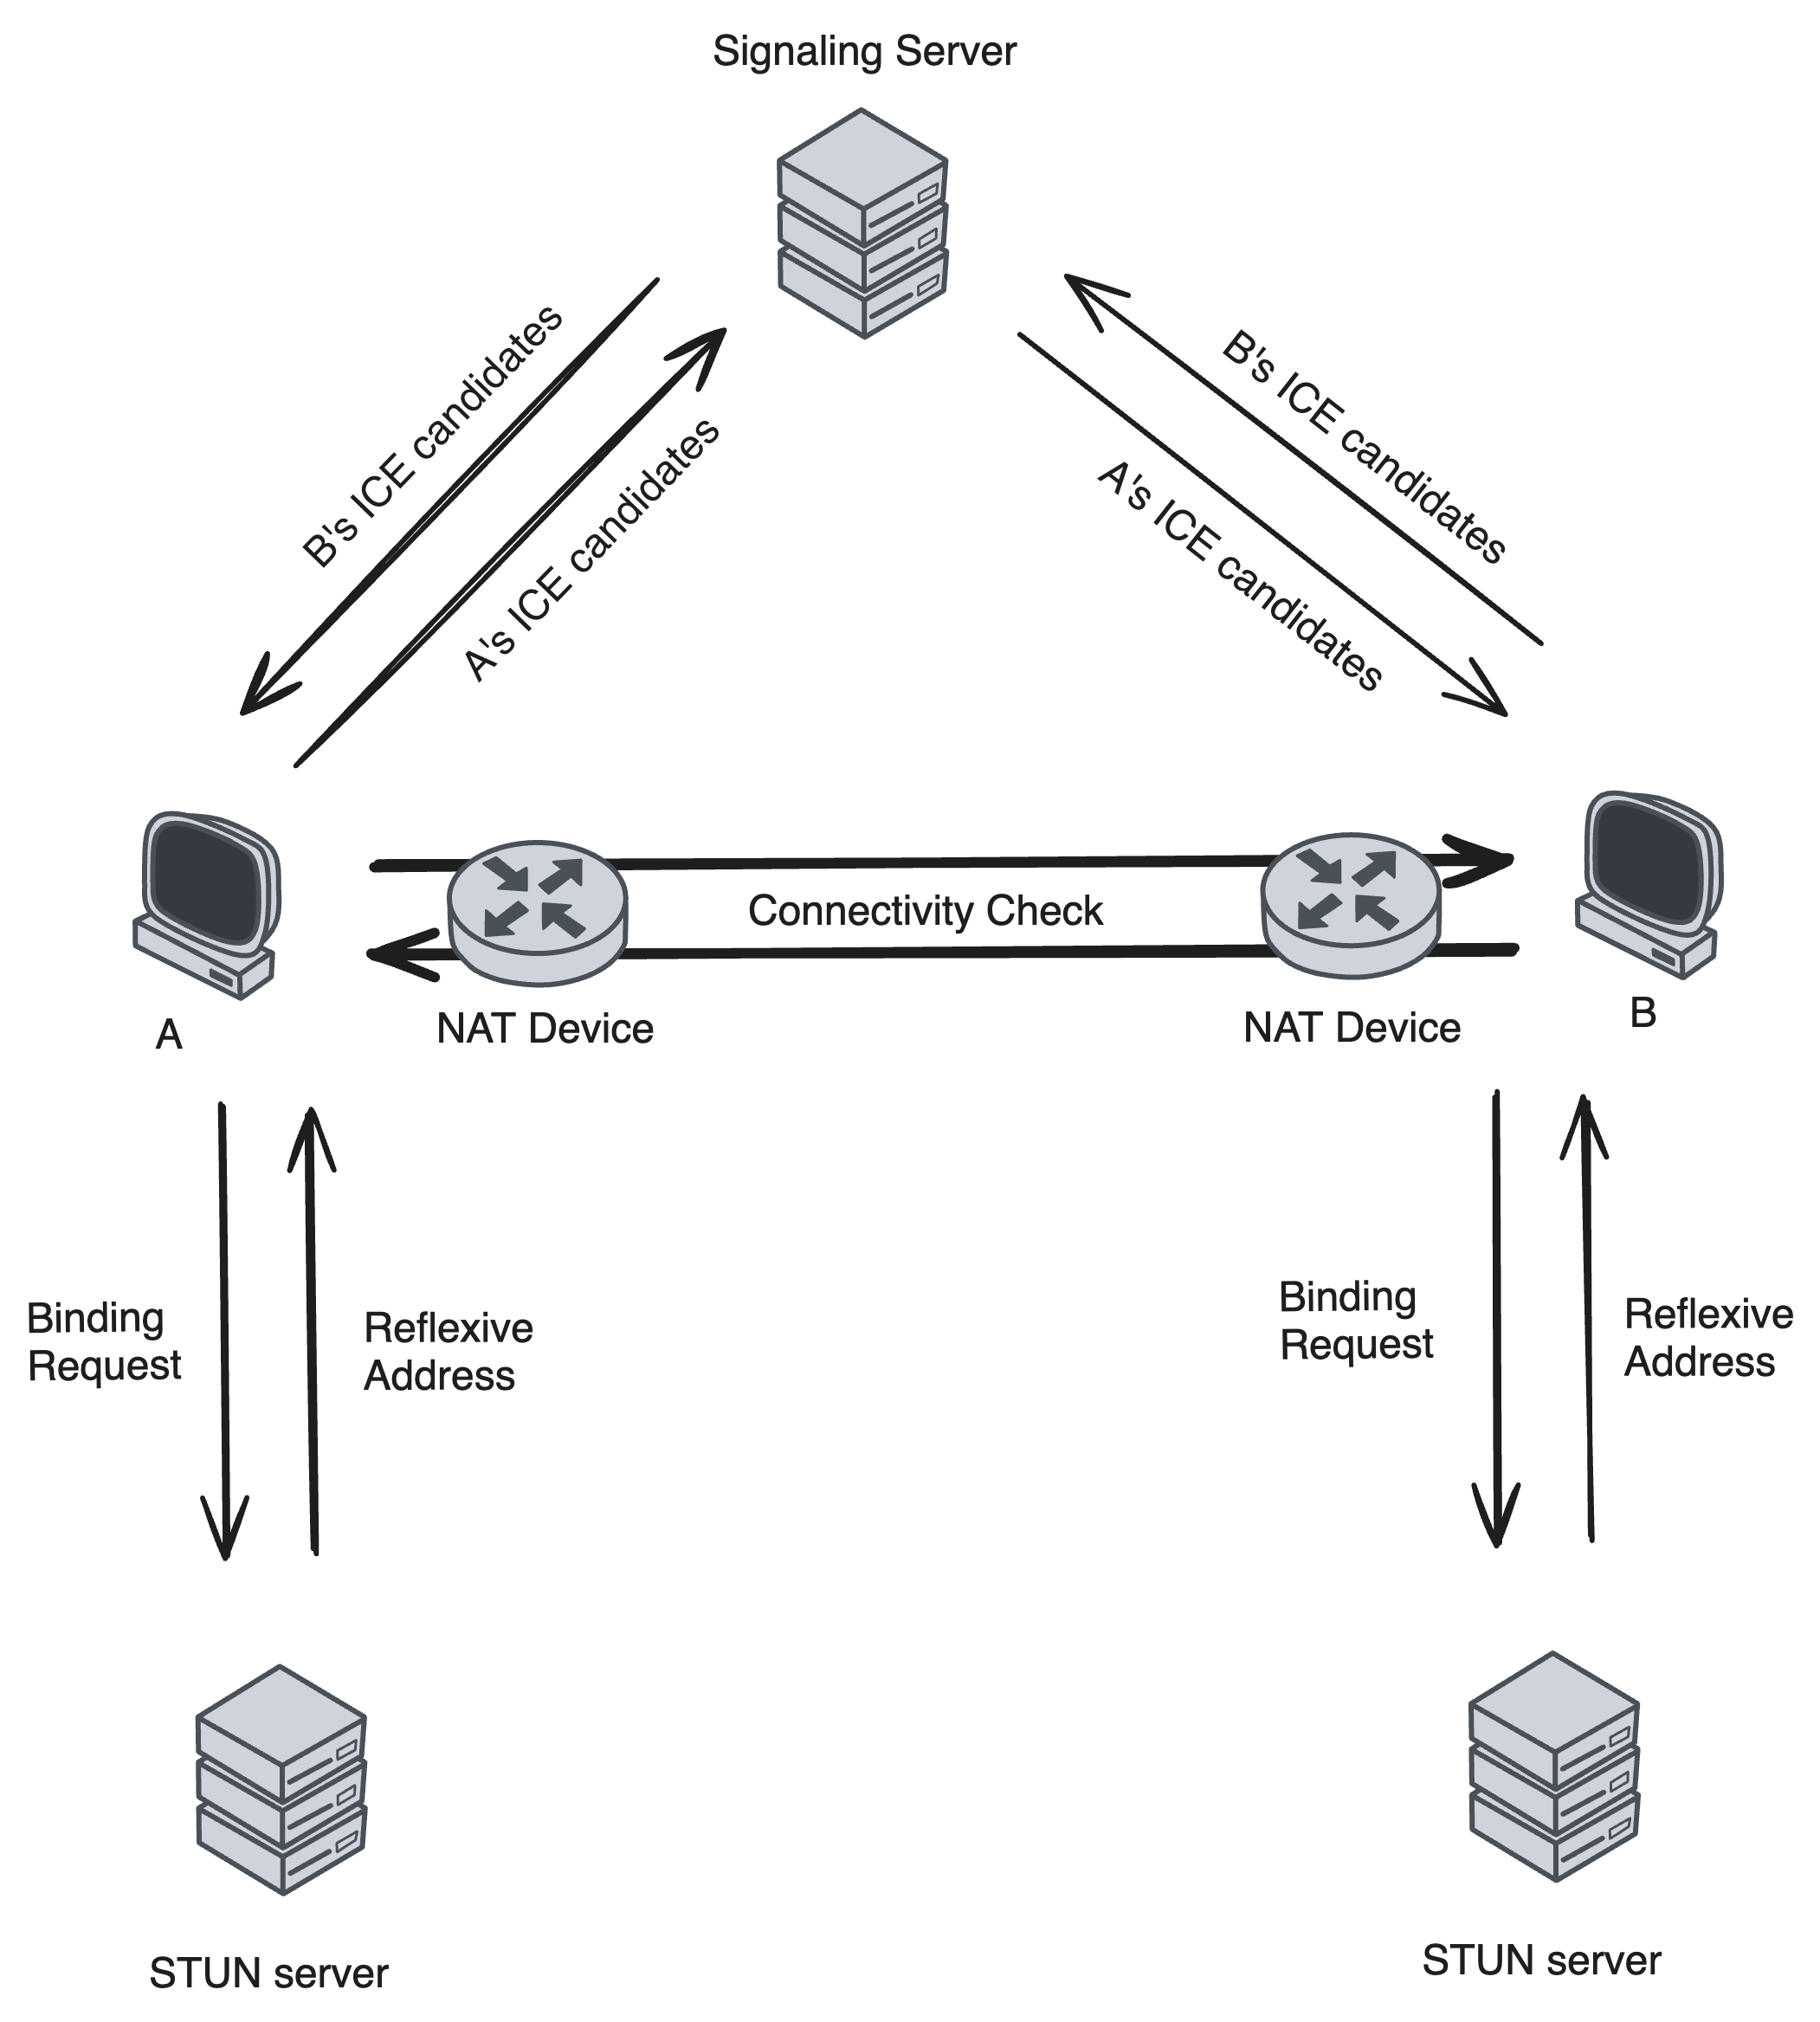
\includegraphics[width=\linewidth]{figs/ice.png}
  \caption{ICEプロトコルによるP2P通信確立の手順}
  \label{fig:ice}
\end{figure}
UDPにおいて,最適なアドレスペアの選択,NAT越えの手順,失敗時のフォールバックなどP2P通信の確立に必要な仕組みを定義した包括的なプロトコルとしてInteractive Connectivity Establishment(ICE)\cite{rfc8445}が定義されている.ICEプロトコルはWebブラウザでのリアルタイム通信プロトコルWebRTC\cite{webrtc}でも利用されており,多くのP2P通信を利用するアプリケーションはICEプロトコルに基づいている.ICEプロトコルによるP2P通信確立の手順を図~\ref{fig:ice}に示す.

\subsection{その他の先行事例}
ICEプロトコルをTCPに応用したTCP Candidates with ICE\cite{rfc6544}が定義されている.

2023年7月にはQUIC上でP2P通信を確立するための包括的なプロトコルP2P QUIC\cite{p2p_quic}のドラフトがIETFに提出されたが,2024年1月に期限切れになっている.
